\mysubsectionformatted{Design Pattern Repository}
\myparagraph{
    Questo design pattern viene usato se, ad esempio, si vuole accedere a una base di dati persistenti.
    
    \begin{tcolorbox}[colback=blue!5!white, colframe=blue!75!black]
        Il pattern fornisce un'illusione di una collezione in memoria per ogni tipo di oggetto persistente che
        richiede l'accesso globale. L'accesso avviene tramite un'interfaccia che definisce delle operazioni per
        aggiungere, rimuovere o ricercare oggetti. Queste operazioni incapsulano l'accesso effettivo alla rappresentazione
        dei dati.
    \end{tcolorbox}
    \vspace{0.1cm}

    \begin{center}
        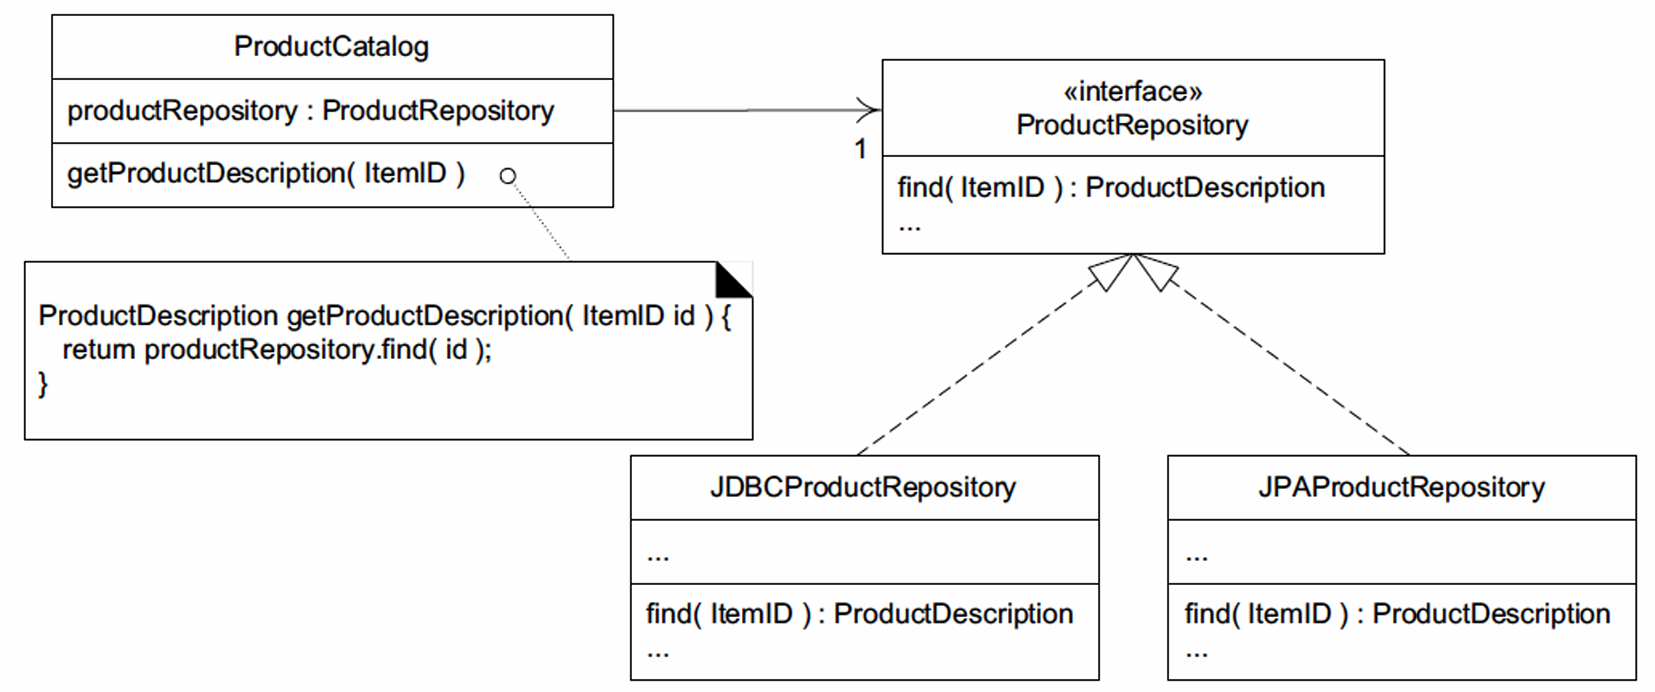
\includegraphics[scale=0.27]{Esercitazione - Design Patterns/repository_pattern.png}
    \end{center}

    In questo esempio abbiamo 3 componenti:
    \begin{enumerate}
        \item \textbf{ProductRepository} è l'interfaccia che funge da repository dei prodotti, viene usata per
        accedere alle informazioni di ciascun prodotto. tramite il metodo \textbf{find()}.
        \item \textbf{JDBCProductRepository} e \textbf{JPAProductRepository} sono delle\\ repository
        contenenti le informazioni.
        \item \textbf{ProductCatalog} è una classe che tramite l'\textit{ItemID} può ottenere la descrizione della
        repository corrispondente.
    \end{enumerate}
    \newpage
}